\documentclass[11pt]{article}
\usepackage{fullpage}
\usepackage{amsthm}

\usepackage{amsthm,amsmath,amsfonts,amssymb,amstext,enumitem}
\usepackage{latexsym,ifthen,url,rotating,graphicx}
\usepackage{listings}
\usepackage{tikz}
\usetikzlibrary{arrows,shapes,positioning,fit}
\usepackage{graphicx}
\usepackage[font=small,labelfont=bf]{caption}



% --- -----------------------------------------------------------------
% --- Document-specific definitions.
% --- -----------------------------------------------------------------
\lstset{
    columns=fixed,
    literate={—}{{---}}1 {…}{{...}}1
}

\newcommand{\todo}[1]{{\color{red}[TODO:{#1}]}}

\newtheorem{problem}{Problem}
\newtheorem{corollary}{Corollary}
\newtheorem{fact}{Fact}
\newtheorem{exercise}{Exercise}
\newtheorem{theorem}{Theorem}
\newtheorem{definition}{Definition}
\newtheorem{notation}{Notation}
\newtheorem{lemma}{Lemma}
\newtheorem{example}{Example}

\newcommand{\getsr}
  {{\:\stackrel{\raisebox{-2pt}{${\scriptscriptstyle \hspace{0.2em}\$}$}}
   {\leftarrow}\:}}
\newcommand{\points}[1]{\textbf{({#1} pts)}}

\newcommand{\Colon}{\ : \ }
\newcommand{\st}{\mathsf{state}}
\newcommand{\msgs}{\mathcal{M}}
\newcommand{\ctxts}{\mathcal{C}}
\newcommand{\keys}{\mathcal{K}}
\newcommand{\kg}{\mathcal{K}}
\newcommand{\enc}{E}
\newcommand{\dec}{E^{-1}}
\newcommand{\MAC}{\mathrm{MAC}}
\newcommand{\RMAC}{\mathrm{RMAC}}

\newcommand{\pk}{pk}
\newcommand{\sk}{sk}

\newcommand{\calD}{\mathcal{D}}
\newcommand{\AES}{\mathsf{AES}}

\newcommand{\algorithm}[1]{\textbf{Alg} {#1}}

\newcommand{\calO}{\mathcal{O}}

\newcommand{\dlog}{\mathrm{dlog}}

\newcommand{\Adv}{\mathbf{Adv}}
\newcommand{\AdvPRF}[2]{\Adv^{\mathrm{prf}}_{#1}({#2})}
\newcommand{\AdvPRG}[2]{\Adv^{\mathrm{prg}}_{#1}({#2})}
\newcommand{\AdvCPA}[2]{\Adv^{\mathrm{ind{-}cpa}}_{#1}({#2})}
\newcommand{\AdvCCA}[2]{\Adv^{\mathrm{ind{-}cca}}_{#1}({#2})}
\newcommand{\AdvKR}[2]{\Adv^{\mathrm{kr}}_{#1}({#2})}
\newcommand{\AdvCKR}[2]{\Adv^{\mathrm{ckr}}_{#1}({#2})}
\newcommand{\AdvRMR}[2]{\Adv^{\mathrm{rmr}}_{#1}({#2})}
\newcommand{\AdvCR}[2]{\Adv^{\mathrm{cr}}_{#1}({#2})}
\newcommand{\AdvUFCMA}[2]{\Adv^{\textrm{uf{-}cma}}_{#1}({#2})}
\newcommand{\AdvDL}[2]{\Adv^{\mathrm{dl}}_{#1}({#2})}

\newcommand{\Exp}{\mathbf{Exp}}
\newcommand{\ExpOW}[1]{\Exp^{\mathrm{ow}}({#1})}
\newcommand{\ExpCKR}[2]{\Exp^{\mathrm{ckr}}_{#1}({#2})}
\newcommand{\ExpRMR}[2]{\Exp^{\mathrm{rmr}}_{#1}({#2})}

\newcommand{\concat}{{\,\|\,}}
\newcommand{\xor}{\oplus}
\newcommand{\bits}{\{0,1\}}

\newcommand{\tcolh}{T^{\mathrm{col}}_h}
\newcommand{\tcolH}{T^{\mathrm{col}}_{H^2}}
\newcommand{\Hcomb}{H^{1\|2}}
\newcommand{\Hxor}{H^{1\oplus2}}

\newcommand{\EXP}{\textrm{EXP}}
\newcommand{\MODEXP}{\textrm{MOD{-}EXP}}
\newcommand{\ADD}{\textrm{ADD}}
\newcommand{\MULTIMODEXP}{\textrm{MULTI{-}MOD{-}EXP}}
\newcommand{\MUL}{\textrm{MUL}}
\newcommand{\MOD}{\textrm{MOD}}

\newcommand{\GG}{\mathbb{G}}
\newcommand{\ZZ}{\mathbb{Z}}

\newcommand{\bK}{\mathbf{K}}
\newcommand{\bU}{\mathbf{U}}
\newcommand{\bM}{\mathbf{M}}
\newcommand{\bC}{\mathbf{C}}

\newcommand{\rvrange}{\mathcal{R}}
\newcommand{\rspace}{\mathcal{C}}

\newcommand{\hatalpha}{\hat{\alpha}}

\newcommand{\otp}{\mathrm{OTP}}

\newcommand{\Img}{\mathrm{Im}}

\newcommand{\heading}[1]{\smallskip\noindent\textsc{#1}}
% --- -----------------------------------------------------------------
% --- Lecture notes formatting macros
% --- -----------------------------------------------------------------

%
% The following commands set up the lecnum (lecture number)
% counter and make various numbering schemes work relative
% to the lecture number.
%
\newcounter{lecnum}
%\renewcommand{\thepage}{\thelecnum-\arabic{page}}
\renewcommand{\thesection}{\thelecnum.\arabic{section}}
\renewcommand{\theexercise}{\thelecnum.\arabic{exercise}}
\renewcommand{\theexample}{\thelecnum.\arabic{example}}
\renewcommand{\thedefinition}{\thelecnum.\arabic{definition}}
\renewcommand{\theequation}{\thelecnum.\arabic{equation}}
\renewcommand{\thefigure}{\thelecnum.\arabic{figure}}
\renewcommand{\thefact}{\thelecnum.\arabic{fact}}
\renewcommand{\thetable}{\thelecnum.\arabic{table}}


%
% The following macro is used to generate the header.
%
\newcommand{\lecture}[2]{
   %\pagestyle{myheadings}
   %\thispagestyle{plain}
   \newpage
   \setcounter{lecnum}{#1}
   \setcounter{page}{1}
   \noindent
   \begin{center}
   \framebox{
      \vbox{\vspace{2mm}
    \hbox to 6.28in { {\bf CMSC 28400 Introduction to Cryptography
                        \hfill Autumn 2020} }
       \vspace{4mm}
       \hbox to 6.28in { {\Large \hfill #2 \hfill} }
       \vspace{2mm}
       \hbox to 6.28in { {\it Instructor: David Cash} \hfill }
      \vspace{2mm}}
   }
   \end{center}
   %\markboth{Lecture #1: #2}{Lecture #1: #2}
   \vspace*{4mm}
}





% --- -----------------------------------------------------------------
% --- The document starts here.
% --- -----------------------------------------------------------------
\begin{document}
%\lecture{**LECTURE-NUMBER**}{**DATE**}{**LECTURER**}{**SCRIBE**}
\lecture{3}{Notes \#3: Stream Ciphers and Computational Security}

%\tableofcontents
%\noindent\hrulefill
%\bigskip

\section{Limitations of the One-Time Pad}

In the last notes we analyzed the One-Time Pad (OTP) cipher, which had a lot
going for it: An implementation should be very fast, since it's just applying
exclusive-OR on two strings, and intuitively-strong security was proved. 
However, while the OTP has been used in the past\footnote{You may
enjoy reading about the
\url{https://en.wikipedia.org/wiki/Venona_project}{Venona Project}, where
American agencies were able to decrypt Soviet OTP-encrypted messages from the
40's to the 80's.}, the OTP itself is not frequently used today, at least not
in the form we saw. This is due to a few reasons:

\heading{Long keys.} To encrypt a message $m$, the OTP requires a key of the
same length. If $m$ is a single credit-card number this may be okay, but to
encrypt the large amount of traffic on the Internet, this is problematic. The
key needs to be transmitted out-of-band, and doing so is typically expensive.
Classically, this meant sending someone with a briefcase of books of keys.  In
the modern setting, we do this via something called \emph{key exchange}, which
we will cover in the second half of the course. Key exchange runs quickly
enough to transmit short keys on any modern laptop, but it's not fast enough to
run for very large keys.

\heading{One-time security.} As we saw before, the OTP loses security if a key
is used twice. One could simply avoid doing so, but then the key-length problem
bites again. We'd like to be able to encrypt multiple times with the same key
if possible, and get some meaningful security.

\heading{Malleability.} This issue is more subtle, but is very relevant in
practice. Suppose the OTP is being used to encrypt a web session, and an
attacker completely controls a router in the middle, with the ability to change
the bits of the traffic however it likes. A ciphertext $c = k\oplus m$ is sent.
Then the attacker is able to modify $c$ so that \emph{the receiver will recover
a message other than $m$}, and moreover the attacker can control what is
received in a predictable way. For example, suppose the attacker flips the
first bit of $c$; call the result $c'$.  If the receiver decrypts $c'$, they'll
recover $m$, except with the first bit flipped.

\smallskip

This type of attack shows that the OTP is \emph{malleable}, in the language
of modern cryptography. It may look a little strange, but malleability attacks
lead to practical vulnerabilities all the time!

\subsection{Our Plan}

The above issues (long keys, one-time security, malleability) will guide our
development of practical encryption methods for the next few weeks. These notes
will begin addressing the first issue. In the next section we'll prove that
\emph{any} cipher unavoidably has long keys if we require it to be perfectly
secret. In the following sections we'll look at something called a \emph{stream
cipher}, which is used to ``stretch'' a short key, and discuss their security.
In the next set of notes we'll get back to applying stream ciphers to
encryption.
The latter two issues require more work and will be addressed in the next two
weeks.

\section{Perfectly Secret Ciphers Must Have $|\keys| \geq |\msgs|$}

The OTP has key as long as the messages. At first glance, one may hope to
develop a different perfectly-secret cipher that has a shorter key.  The
following theorem shows this is in some sense impossible (and is precisely
impossible if one insists that $\keys$ is a set of fixed-length bitstrings).
\begin{theorem}
    Suppose a cipher $\enc : \keys\times\msgs \to \ctxts$ is perfectly secret.
    Then $|\keys| \geq |\msgs|$.
\end{theorem}
\begin{proof}
    We prove the contrapositive, meaning we show that if $|\keys| < |\msgs|$,
    then $E$ is \emph{not} perfectly secret. In order to show $E$ is not
    perfectly secret, we find some $m_0,m_1\in\msgs$ and $c\in\ctxts$ such that
    \begin{align}\label{neqprob}
        \Pr[\enc(\bK,m_0) = c] \neq \Pr[\enc(\bK,m_1) = c],
    \end{align}
    where $\bK$ is uniform on $\keys$.

    We start by taking $c\in\ctxts$ to be an arbitrary element of the image of
    $E$ (so, we know that $E(k,m)=c$ for some $k\in\keys,m\in\msgs$, but we
    don't care how its picked beyond that).

    Define the set $X$ of ``all possible decryptions of $c$'' as
    \[
        X = \{E^{-1}(k,c) \ | \ k\in\keys \}.
    \]
    Notice that $|X| \leq |\keys|$, because at most one element is added to $X$
    per element of $\keys$ (it might be less because we might add the same
    element twice). By our choice of $c$ we also have that $X$ is non-empty;
    pick some arbitrary $m_1\in X$.

    Since $|X| \leq |\keys|$, and we assumed $|\keys| < |\msgs|$, we have
    $|X| \leq |\msgs|$. Therefore $X$ does not contain all of $\msgs$, and
    can choose some $m_0 \in \msgs$ that is not in $X$.
    The following diagram shows the relationship between $c,m_1$ and $m_0$.
    \begin{center}
        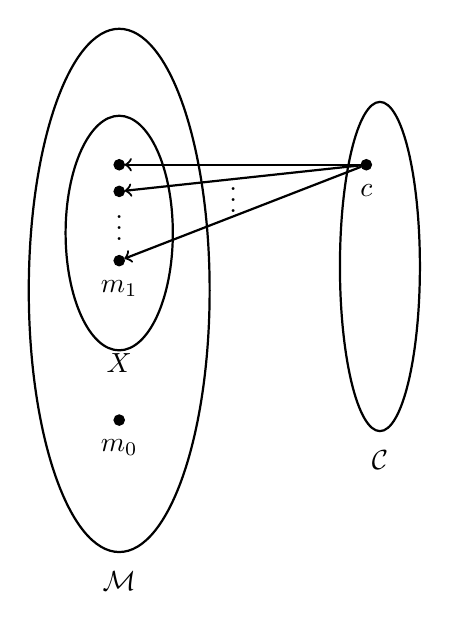
\begin{tikzpicture}
            \tikzstyle{connect}=[circle, draw, thin,fill=black, scale=0.4]
            \tikzstyle{every path}=[thick]
            \tikzstyle{rotor}=[very thick, rounded corners]
            \tikzstyle{input}=[circle,draw,scale=.7]
            \tikzstyle{internalwire}=[thick,darkgray]

            \node[connect] (m1) {};
            \node[connect, below=.2cm of m1] (m2) {};
            \node[below=-.1cm of m2] (dots) {$\vdots$};
            \node[connect, below=.05cm of dots] (m3) {};
            \node[below=.05cm of m3] (m3label) {$m_1$};
            \node[shape=ellipse,draw,fit={(m1) (m3label)}] (X) {};
            \node[below=-.1cm of X] (Xlabel) {$X$};

            \node[connect, below=.4cm of Xlabel] (m0) {};
            \node[below=.05cm of m0] (m0label) {$m_0$};

            \node[shape=ellipse,draw,minimum width=1.5cm,fit={(X) (m0label)}] (msgs) {};
            \node[below=.1cm of msgs] {$\msgs$};

            \node[connect, right=3cm of m1] (c) {};
            \node[below=.05cm of c] (clabel) {$c$};
            \node[right=3cm of Xlabel] (cinvis) {};
            \node[shape=ellipse,draw,minimum width=1cm,fit={(c) (cinvis)}] (ctxts) {};
            \node[below=.1cm of ctxts] {$\ctxts$};

            \draw [->] (c) -- (m1);
            \draw [->] (c) -- (m2);
            \node[right=1.2cm of m2] {$\vdots$};
            \draw [->] (c) -- (m3);

        \end{tikzpicture}
    \end{center}
    We have chosen our $m_0,m_1$, and $c$. It remains to verify that
    (\ref{neqprob}) holds. This follows by two observations:
    \begin{itemize}
        \item $\Pr[E(\bK,m_0)=c] = 0$, because there is no key $k$ such
            that $E(k,m_0)=c$.
        \item $\Pr[E(\bK,m_1)=c] \geq 1/|\keys| > 0$, because there
            is at least one key $k$ such that $E(k,m_1)=c$.
    \end{itemize}
    This shows the probabilities are not equal and completes the proof.
\end{proof}


\section{Plan:  ``Psuedo''-One-Time Pad Encryption}

In the last section we showed that \emph{any} perfectly secret cipher
$E:\keys\times\msgs\to\ctxts$ must satisfy $|\keys| \geq |\msgs|$.
Thus for each $n$, $\otp_n$ is ``optimal'' in terms of key-length
for perfectly-secret ciphers.

In practice the one-time pad is rarely used because exchanging the key is
cumbersome. In practice one resolves this barrier by giving up on perfect
secrecy, and using a weaker-but-good-enough notion of security. In order
to work with a shorter key, we'll look for a function that can ``securely
stretch'' a short key into a long one. More formally we'll want some
\[
    G:\bits^n \to \bits^\ell
\]
where $\ell \ll n$; For example, $n=256$ and $\ell$ practically-infinite (like
$\ell=2^{64}$) is typical. (Of course we need that we evaluate $G$ efficiently
so we can actually use it; Typically we want to be able to compute the bits of
$G$ from the first to however many we need, rather than needing to compute them
all at the same time, up front.)

Functions $G$ for stretching keys will be called \emph{pseudorandom generators}
of \emph{stream ciphers} (the two names mean the same thing for us; The applied
community often uses ``stream cipher'' while the theoretical community
typically uses ``pseudorandom generators''). Note that stream ciphers are not
really \emph{ciphers} as defined earlier, since we they only take one input,
and we are not requiring them to satisfy any one-to-one condition.

We will use $G$ to build a cipher as follows:
\begin{definition}
    Let $n,\ell$ be positive integers, and let
    $G:\bits^n\to\bits^\ell$ be a function. Define the
    \emph{$G$-pseudo-one-time-pad cipher}
    \[
        \otp_G:\bits^n\times\bits^\ell\to\bits^\ell
    \]
    defined by
    \[
        \otp_G(k,m) = G(k)\oplus m.
    \]
\end{definition}

First, the bad news.
\begin{theorem}
    Let $n,\ell$ be positive integers, and let
    $G:\bits^n\to\bits^\ell$ be a function. If $\ell > n$ then
    $\otp_G$ is not perfectly secret.
\end{theorem}
This is true because there are fewer keys ($2^n$) than messages ($2^\ell$) when
$\ell > n$.

The good news is that, practically speaking, we can still do very well; We just
need to be careful about how we design $G$, and then also careful about what
level of security we are actually achieving. Thus we shift our focus from
$\otp_G$ to $G$ itself for now. In future lectures we'll give a definition to
analyze $\otp_G$.

\section{Defining Security of Pseudorandom Generators}

We want a pseudorandom generator that will work well in stretching a key to use
in place of a one-time pad. A natural requirement is that the output of $G$,
when run on a uniformly random input, should pass an array of statistical
tests. The numbers of zeros and ones should be approximately balanced, like a
random string, and there should be typical runs of consecutive zeros and ones,
and so on.

Typically scientific applications of pseudorandom generators get by with this
sort of thinking. Since they employ the random bits in simulating physical
phenomena, they only need to worry about a specific model behaving normally
on the output bits.
As we will see, our situation is however much more demanding. 

Defining the quality of pseudorandom bits is tricky. Even if $G$ always
outputs something very non-random (like the all-zeros string), we can't
for sure say that it's \emph{not} random; After all, for a uniform sample,
all outcomes are equally likely, including the all-zeros string.
Instead of looking at individual strings, we need to look at the
\emph{distribution} output by $G$.

Let us first give a definition to measure how effective a statistical test
(denoted $\calD$ below, for ``distinguisher'') is against a pseudorandom
generator.
\begin{definition}
    Let $G:\bits^n\to\bits^\ell$ and $\calD:\bits^\ell \to \bits$ be functions
    and let $\bK$ be uniform on $\bits^n$ and $\bU$ be uniform on $\bits^\ell$.
    Then we define the \emph{(pseudorandom generator) distinguishing advantage
    of $\calD$ against $G$} to be
    \[
        \AdvPRG{G}{\calD} =
        \left|\Pr[\calD(G(\bK))=1]-\Pr[\calD(\bU)=1]\right|.
    \]
\end{definition}
The definition is useful because, for a specific $G$ and any test $\calD$, it
assigns a number between $0$ and $1$ (the higher the better $\calD$ is).
Thus we can compare distinguishers, and speak of how well $G$ passes
statistical tests.

Let's do a warm-up example with the definition, and then return
to interpreting the definition later. 
\begin{example}
    Let $G:\bits^n\to\bits^{n+1}$ be defined by $G(k)=k\|0$, where we use
    the symbol $\|$ to denote string concatenation (in words, $G$ simply
    puts a zero on the end of $k$). For any reasonable definition of
    pseudorandom generation, $G$ should fail -- It's just adding a zero
    bit!

    To formalize the failure of $G$, take
    \[
        \calD(w) =
        \begin{cases}
            1 & \text{if $w$ ends in $0$}\\
            0 & \text{otherwise}
        \end{cases}.
    \]
    Then we claim
    \[
        \AdvPRG{G}{\calD} = \frac{1}{2}.
    \]
    We can compute this by looking at the two probabilities in the
    definition above:
    \[
        \Pr[\calD(G(\bK))=1] = 1
    \]
    because $G(\bK)$ will end in a $0$ with probability $1$.
    Next,
    \[
        \Pr[\calD(\bU)=1] = \frac{1}{2}.
    \]
    This latter probability is $1/2$ because a random string ends in
    $0$ with probability $1/2$.
\end{example}
We note from this example that $G$ is a terrible pseudorandom generator,
and this distinguisher only achieves advantage $1/2$; Thus we should
consider such an advantage to ``very large''.

\begin{exercise}
    Let $G:\bits^n\to\bits^{2n}$ be defined by $G(k)=k\|k$ (i.e it copies
    $k$ twice). Find a good distinguisher $\calD$ for $G$ and calculate
    $\AdvPRG{G}{\calD}$.
\end{exercise}

Armed with this definition we can ask that $\AdvPRG{G}{\calD}$ be ``low''
for \emph{any} distinguisher $\calD$. If we're feeling ambitious, we
could even ask that it's always zero. Unfortunately this is impossible,
as we now prove.
\begin{theorem}
    Let $n,\ell$ be positive integers with $\ell>n$, and let
    $G:\bits^n\to\bits^\ell$ be a function. Then there exists
    $\calD:\bits^\ell\in\bits$ such that
    \[
        \AdvPRG{G}{\calD} \geq 1- \frac{2^n}{2^\ell} \geq \frac{1}{2}.
    \]
\end{theorem}
\begin{proof}
    Let $\Img\ G$ be the image of $G$, i.e. $\Img\ G = \{G(k) \ :\
    k\in\bits^n\}$.  The function $\calD:\bits^\ell\to\bits$ is defined by
    \[
        \calD(w) =
        \begin{cases}
            1 & \text{if $w\in\Img\ G$} \\
            0 & \text{otherwise}
        \end{cases}.
    \]
    
    To analyze $\calD$ we need two observations about $\Img\ G$. First, the
    random variable $G(\bK)$ is always in $\Img\ G$. Second, $|\Img\ G| \leq
    2^n$, because each $k\in\bits^n$ adds at most one element to the image, and
    there are $2^n$ such $k$ (it may be less when $G$ is not one-to-one).

    Then letting $\bK,\bU$ as in the theorem,
    \[
        \Pr[\calD(G(\bK))=1]=1
    \]
    because $G(\bK)$ is always in the image of $G$. On the other hand,
    \[
        \Pr[\calD(\bU)=1] \leq \frac{2^n}{2^\ell},
    \]
    because $\calD(\bU)=1$ is equivalent to $\bU\in\Img\ G$, which happens
    with probability $|\Img\ G|/2^\ell$. By our observation on the size
    $\Img\ G$, this probability is at most $\frac{2^n}{2^\ell}$. Finally,
    plug these in to get
    \begin{align*}
        \AdvPRG{G}{\calD} & =  
        |\Pr[\calD(G(\bK))=1] - \Pr[\calD(\bU)=1]| \\
        & \geq 
        \Pr[\calD(G(\bK))=1] - \Pr[\calD(\bU)=1] \\
        & \geq 
         1 - \frac{2^n}{2^\ell} \geq 1 - \frac{1}{2} = \frac{1}{2}.
    \end{align*}
\end{proof}

\begin{exercise}
    Let $G:\bits^n\to\bits^\ell$. Show that for \emph{any}
    $\calD:\bits^\ell\to\bits$,
    \[
        0 < \AdvPRG{G}{\calD} < 1.
    \]
    That is, no distinguisher can be ``perfectly correct'' or ``perfectly
    incorrect''.
\end{exercise}

\subsection{The Computational View of Security}

On the one hand, this theorem is bad for us, because it says that there will
always be a distinguisher $\calD$ that can detect a pattern in $G$.  However,
in practical terms this distinguisher is not so concerning; Unless we have some
insight into the workings of $G$, to implement the $\calD$ from the theorem on
a computer, we need to test if an input string $w$ is in the image of $G$. To
do this, we would need to loop over \emph{all} $k\in\bits^n$ and test if $G(k)$
is equal to $w$. 

This resulting program would run \emph{exponential time} $2^n$.  For small $n$
like $n=30$ or $40$ this would run relatively quickly.  But for $n=60$ or so
this would easily overwhelm a personal computer. And for $n=128$, it is
commonly thought that such a computation would be beyond even the strongest
agencies on earth.  For $n=256$, such a computation seems \emph{beyond the
physical limits of the universe}, as some estimates put the number of atoms in
the universe at around $2^{256}$.

\begin{exercise}
    To get an idea for the scaling involved, try estimating the cost to
    implement a $2^{128}$-level computation in one year. Find a 
    recent graphics card, and estimate the number of operations
    per year that it can compute (taking it simply the number of cores
    times the clock speed). Assuming generously that one key can be tried
    per cycle per core, calculate the number of graphics cards (and hence
    the cost) required to try all $128$-bit keys.
\end{exercise}

In practice one typically designs a $G$ and tries to find efficient
distinguishing attacks. For an attack $\calD$ under consideration, we
care about both its runtime $T$ and its advantage $\AdvPRG{G}{\calD}$.
An example security target for $G$ might be:
\begin{align}\label{eq:bound}
    \text{For all $\calD$ with running time $2^{128}$ or less,
$\AdvPRG{G}{\calD}\leq 1/2^{128}$.}
\end{align}
Note that we've allowed a huge running time and still want an incredibly small
advantage. The small advantage is to ensure that even after using $G$ an
astronomical number of times, any detectable bias should still be very, very
small.

Note that we have been informal with our notion of ``running time.'' We will
leave this informal for the purposes of this course, but if we really wanted to
formalize it we could turn to models of computation like Turing Machines and
circuit families; This course is designed to work without knowledge of those
concepts.  There are some interesting details to sort out there, but we'll get
by just fine without commenting on that again.  One thing we \emph{can't} do,
however, is use big-Oh analysis: We don't care about limits going to infinity.
We will care about how hard it is to break our constructions.

Finally, we remark on the possibility of finding a good stream cipher $G$ and
then \emph{proving} a statement like that of Equation~\ref{eq:bound}. This
would require somehow analyzing the structure of any possible efficient attack,
and arguing that none could possibly work. Unfortunately, such an argument is
totally beyond the state-of-the-art of theoretical computer science. In fact,
making progress on such questions is one of the central goals of
\emph{computational complexity theory}. You have probably heard of the ``P vs.
NP'' problem, and the same issue is at work here: We have almost no tools for
proving that efficient computation is incapable of doing anything in
particular. This is not great for practice (when do we know if something is
secure?), but it adds quite a bit of mystery to cryptography, since we never
\emph{really} know if there is a more clever attack or not. In any case, it
does not mean that the type of statement above is without value, since it gives
us a standard by which to declare $G$ ``broken,'' should someone present an
attack.


\end{document}

